\chapter{Introduction}

\label{chapter:introduction}

\section{Motivation}

With the recent trend of increasingly large deep learning models achieving
State-Of-The-Art (SOTA) performance on a myriad of Machine Learning (ML) tasks
(Figure \ref{fig:nlp_progress}), several studies argue for focused research into
Explainable Artificial Intelligence (XAI) to address emerging concerns such as
security risks and inductive biases associated with black-box models
\citep{doran2017does,townsend2019extracting,danilevsky2020survey,arrieta2020explainable}.
Of these studies, \citet[Page 4, Section 2.2]{arrieta2020explainable} provide
the following novel definition of XAI based on an extensive literature review of
recent XAI research:

\begin{quote}
  \textit{``Given an audience, an \textbf{explainable} Artificial Intelligence
    is one that produces details or reasons to make its functioning clear or
    easy to understand.''}
\end{quote}

In addition, \citet{arrieta2020explainable} explore and classify a variety of
machine-learning models into transparent and black-box categories depending on
their degrees of transparency. Furthermore, they explore taxonomies of post-hoc
explainability methods aimed at effectively explaining black-box models. Of high
relevance to this study are the local explanations, feature relevance and
explanations by simplification post-hoc explainability techniques.

Through a survey of recent literature on explanations by simplification applied
in the Natural Language Processing (NLP) field, we came across several prominent
studies employing techniques to simplify black-box neural networks into
constituent Finite-State Automata (FAs) and/or Weighted Finite-State Automata
(WFAs)
\citep{schwartz2018sopa,peng2018rational,suresh-etal-2019-distilling,wang2019state,jiang2020cold}.

In this thesis, we build upon the work of \citet{schwartz2018sopa} by further
developing their \textbf{So}ft \textbf{Pa}tterns (SoPa) model; which represents
a hybridized RNN, CNN and Weighted Finite-State Automaton neural network
architecture. We modify the SoPa model by changing key aspects of its
architecture which ultimately allows us to conduct effective explanations by
simplification; which was not possible with the previous SoPa architecture. We
abbreviate this modified model as \textbf{SoPa++}, which signifies an
improvement or major modification to the SoPa model. Finally, we evaluate both
the performance and explainability of the SoPa++ model on the Facebook
Multilingual Task Oriented Dialog data set (FMTOD;
\citealt{schuster-etal-2019-cross-lingual}); focusing on the English-language
intent classification task.

\begin{figure}[th]
  \centering
  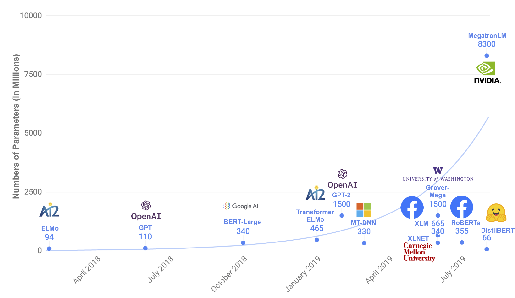
\includegraphics[width=13cm]{pdfs/borrowed/nlp_sota_model_size_progress.pdf}
  \caption{Parameter counts of recently released pre-trained language models
    which showed competitive or SOTA performance when fine-tuned over a range of
    NLP tasks; figure taken from \citet{sanh2019distilbert}}
  \label{fig:nlp_progress}
\end{figure}

\section{Research questions}

With the aforementioned modifications to the SoPa architecture and the
introduction of the SoPa++ architecture, we aim to answer the following three
research questions:

\begin{enumerate}
  \item To what extent does SoPa++ contribute to competitive
  performance\footnote{We define competitive performance as the scenario where a
    mean performance metric on a certain data set falls within the range
    obtained from other recent studies on the same data set} on the FMTOD data
  set?
  \item To what extent does SoPa++ contribute to effective explanations by
  simplification on the FMTOD data set?
  \item What interesting and relevant explanations can SoPa++ provide on the
  FMTOD data set?
\end{enumerate}

\section{Thesis structure}

With the aforementioned research questions, we summarize the structure and
contents of this thesis.

\begin{description}[align=left]
  \item [Chapter 1:] Introduce this thesis, its contents and our research
  questions.
  \item [Chapter 2:] Describe the background concepts utilized in this thesis.
  \item [Chapter 3:] Describe the methodologies pursued in this thesis.
  \item [Chapter 4:] Describe the results obtained from our methodologies.
  \item [Chapter 5:] Discuss the implications of the aforementioned results.
  \item [Chapter 6:] Conclude this thesis by answering the research questions.
  \item [Chapter 7:] Document future work to expand on our research questions.
\end{description}

%%% Local Variables: 
%%% mode: latex
%%% TeX-master: "main"
%%% End: 

% LocalWords:  SOTA XAI explainability NLP Automata FAs WFAs FMTOD th nlp pre
% LocalWords:  sota tterns
